\chapter{Zadanie 7.}
Odporno�� algorytmu przy parametrach $ D = D^{z} = N = N_{u} = 200 $ oraz $ \lambda = 5 $ zbadano dla zerowego zak��cenia(rysunek ~\ref{dmc_szum_0}), sta�ej niezerowej warto�ci zak��cenia, w tym przyk�adzie r�wnej $ \num{0.2} $(rysunek ~\ref{dmc_szum_stale}) oraz zak��cenia rosn�cego liniowo(rysunek ~\ref{dmc_szum_lin}). Zbadano te� r�ne rodzaje szum�w. Jak wida� regulator nie radzi sobie tylko przy du�ym bezwzgl�dnym szumie.

\begin{figure}[b]
\centering
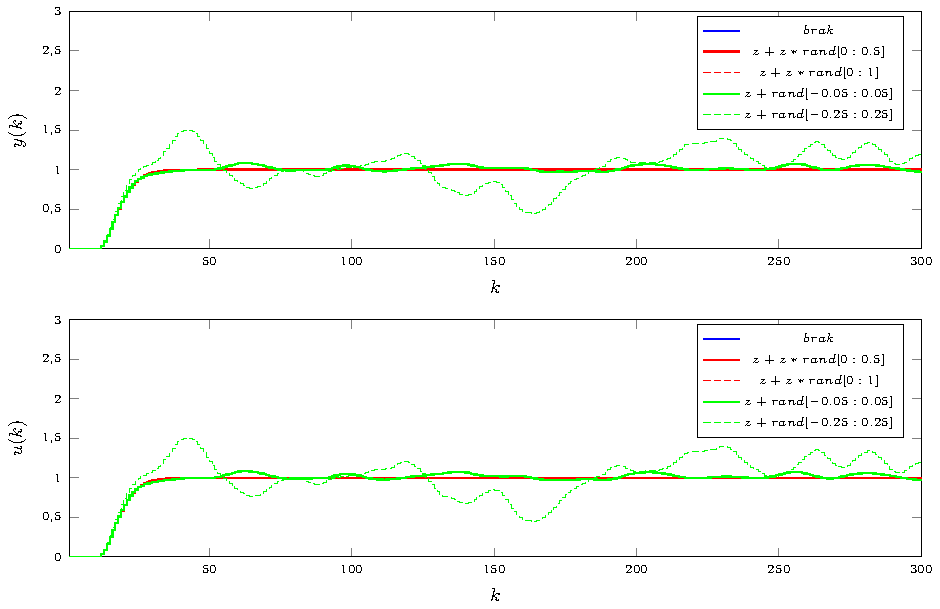
\includegraphics[scale=1.4]{../wykresy_pdf/zad7_dmc_blad1.pdf}
\caption {Symulacja algorytmu DMC dla przy szumie pomiarowym i zerowym zak��ceniu}
\label{dmc_szum_0}
\end{figure}

\begin{figure}[b]
\centering
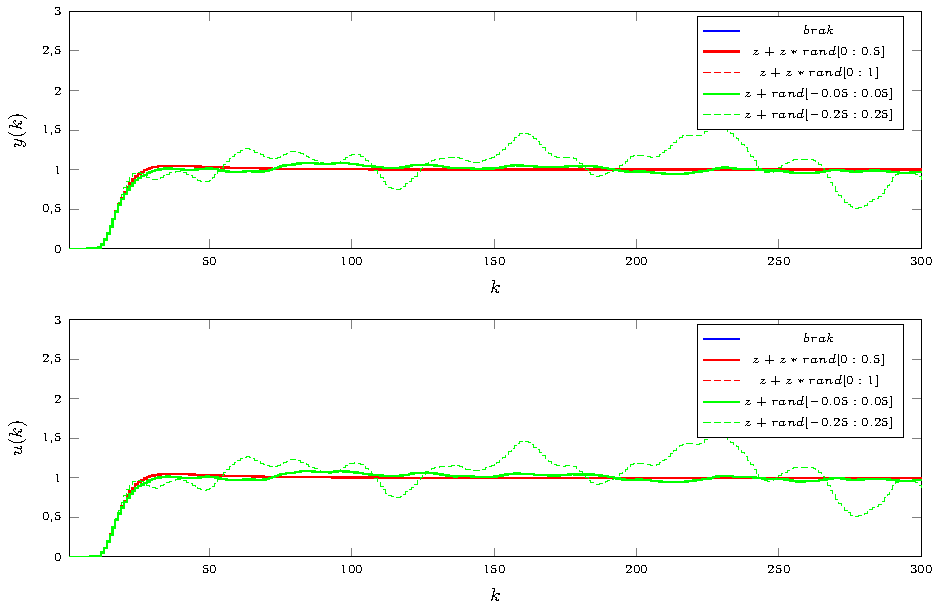
\includegraphics[scale=1.4]{../wykresy_pdf/zad7_dmc_blad2.pdf}
\caption {Symulacja algorytmu DMC dla przy szumie pomiarowym i sta�ym niezerowym zak��ceniu}
\label{dmc_szum_stale}
\end{figure}

\begin{figure}[b]
\centering
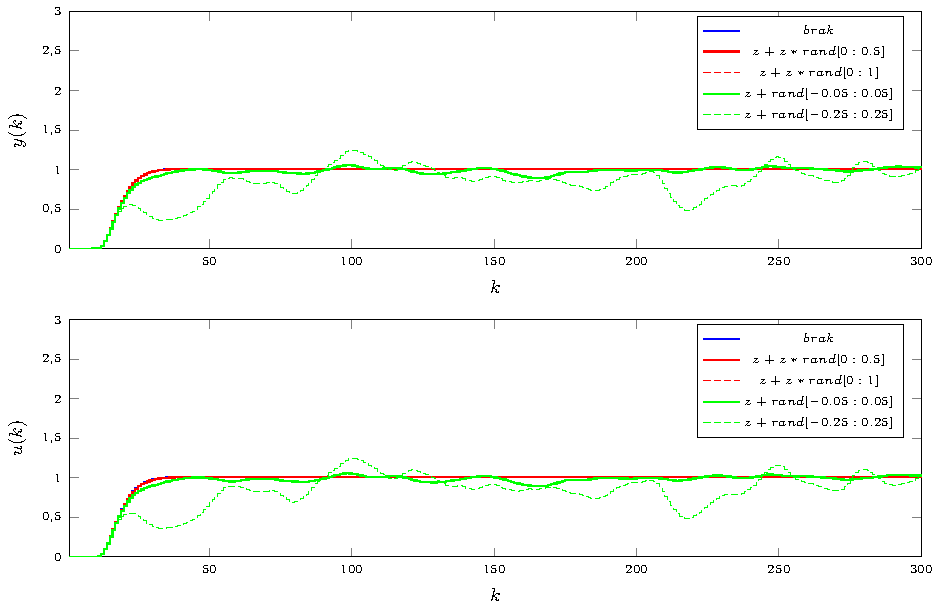
\includegraphics[scale=1.4]{../wykresy_pdf/zad7_dmc_blad3.pdf}
\caption {Symulacja algorytmu DMC dla przy szumie pomiarowym i zak��ceniu rosn�cym liniowo}
\label{dmc_szum_lin}
\end{figure}